%!TEX root=../master.tex

\section{Consumer attacking the electrical company}\label{attacks:consumer_vs_electrical}
This section will contain the attack where the consumer wants to deceive the electrical company into billing for a lower amount than actually consumed.
To facilitate the reader in understanding the details of the attack tree in \cref{report_power_attack_tree} its nodes and sub-\emph{``trees''} will be described below.
In order for an electrical company to bill the consumer, he must first receive information from the smart meter about the consumer's power consumption.

The goal of the consumer is to report at lower power consumption than what is actually measured by the smart meter.
The attack tree describes two different possible attacks that could achieve this goal.


\afterpage{% Insert after the current page
\cleardoublepage
\thispagestyle{plain}
\KOMAoptions{paper=A3,paper=landscape}
\recalctypearea

\begin{figure}
  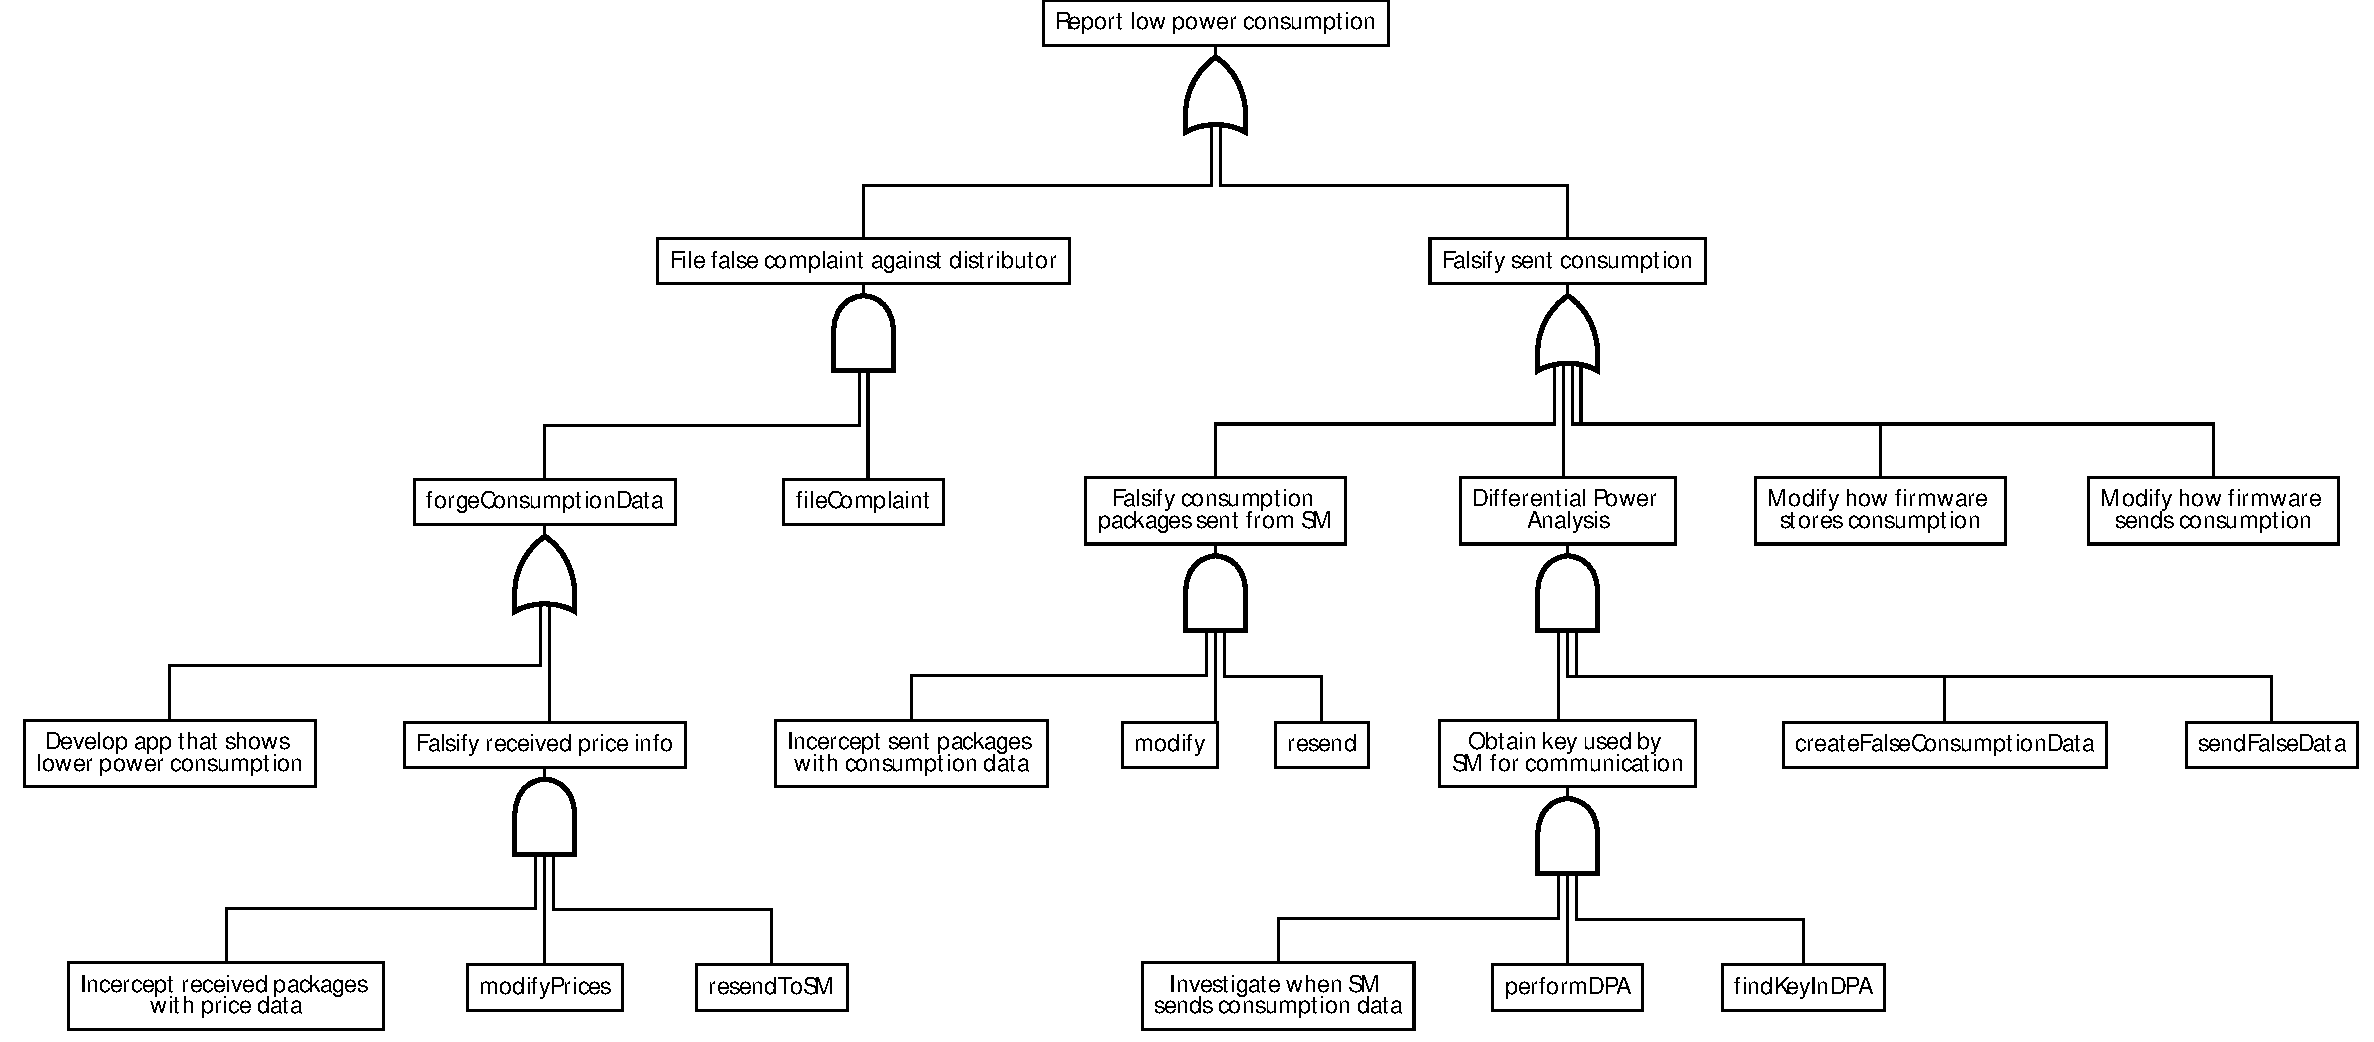
\includegraphics[width=\textwidth]{graphviz/consumer.pdf}
  \caption{The consumer attacking the electrical company by reporting a lower consumption than measured by the smart meter.}
  \label{report_power_attack_tree}
\end{figure}

\cleardoublepage
\KOMAoptions{paper=A4,pagesize}
\recalctypearea
}

\subsection{File false complaint against electrical company}
This attack involves the attacker attempting to prove that the electrical company is billing him for a too large power consumption.
This despite the bill actually corresponding with correct usage and price information.

The project group suggest two different approaches to achieving this goal:
\begin{enumerate}
  \item The user develops an application that mimics an official app describing the power consumption.
  This application will display an incorrectly low information about the consumers power consumption.
  \item The user successfully alters pricing information as received from the electrical company.
  He will want to lower the price locally, such that when he examines his ``expected bill'' the total price will be lower than that billed by the electrical company.
  The attack requires that the consumer is able to modify the prices, e.g. by tampering incoming network packages -- as pictured, as they are received by his smart meter.
  Network attacks will be described in \cref{attacks}.
\end{enumerate}
Both of the above require the user to claim wrong-doing on behalf of the electrical company.
Any one individual might have a problem in assuring the validity of their claim.
However applying this attack on a larger scale will provide a possibly stronger case.

Additionally this type of attack might be carried out by the attacker on other consumers' smart meters, effectively hiding his intent by having multiple unaware consumers complain as well.

\subsection{Falsify sent consumption}
As the attacker (the consumer) is interested in what is reported to his electrical company, he could falsify this information.

In the attack tree, there can be seen four overall methods of achieving this:
\begin{enumerate}
  \item Tampering data sent from/to the smart meter.
  \item Reverse engineering the firmware 
  \item Modifying the firmware in order to change how the consumer's power consumption is stored.
  \item Modifying the firmware in order to change how the consumer's power consumption is sent.
\end{enumerate}

\subsubsection{Tampering}
The goal of the first attack is to intercept the packages sent from the meter, modify them and resend them to the electrical company.
Alternatively the attacker might intercept packages at times where he knows his power consumption to be low and resend them at a later point in time where he knows them to be high.
This is known as a replay attack (see \cref{replay_attack}).

Safeguards against this type of tampering is encryption and authentication. 
These concepts will be discussed in \cref{cryptography}.
Even though the communication between the smart meter and the distributor is both encrypted and authenticated, nothing is guaranteed to be secure.
As discussed in \citet{cryptoenginering}, cryptography is very difficult, and protocols that are regarded as secure may contain a small error that is discovered after several years.
Also the implementation of a cryptographic system determines how secure it is, as well as the surroundings of the system \citep{cryptoenginering}. 
If the surrounding system is leaking left and right, a correctly implemented encryption algorithm can not be blamed.

\subsubsection{Reverse engineering}
By performing reverse engineering the firmware the consumer will possibly get information that enables him to falsify the information sent from the smart meter.
By performing a side-channel attack the consumer could be able to acquire the key(s) which is used to ensure authentication and integrity of sent messages.
This way the consumer could send packages which seem authentic.
Side channel attacks will be discussed in \cref{attack:sidechannel}.

\subsubsection{Modifying firmware}
The final attack(s) we propose include tampering with the smart meter's firmware.
If the consumer is able to change or replace the firmware on the smart meter, he could be able to modify the way that the smart meter either stores or sends power consumption data.
\stefan{ret udetaljeret}